\documentclass[12pt]{article}
\setlength{\oddsidemargin}{0in}
\setlength{\evensidemargin}{0in}
\setlength{\textwidth}{6.5in}
\setlength{\parindent}{0in}
\setlength{\parskip}{\baselineskip}
\usepackage{amsmath,amsfonts,amssymb}
\usepackage{graphicx}
\usepackage{enumitem}
\usepackage[]{algorithmicx}
\usepackage{amsthm}
\usepackage{fancyhdr}
\pagestyle{fancy}
\setlength{\headsep}{36pt}
\usepackage{tkz-berge}
\usetikzlibrary{positioning, automata}

\usepackage{hyperref}

\theoremstyle{remark}
\newtheorem*{solution}{Solution}

\newcommand{\makenonemptybox}[2]{%
%\par\nobreak\vspace{\ht\strutbox}\noindent
\item[]
\fbox{% added -2\fboxrule to specified width to avoid overfull hboxes
% and removed the -2\fboxsep from height specification (image not updated)
% because in MWE 2cm is should be height of contents excluding sep and frame
\parbox[c][#1][t]{\dimexpr\linewidth-2\fboxsep-2\fboxrule}{
  \hrule width \hsize height 0pt
  #2
 }%
}%
\par\vspace{\ht\strutbox}
}
\makeatother

\begin{document}

\lhead{{\bf CSCI 3104, Algorithms \\ Problem Set 9b (51 points)} }
\rhead{Name: Luna McBride \\ ID: 107607144 \\ {\bf Profs.\ Hoenigman \& Agrawal\\ Fall 2019, CU-Boulder}}
\renewcommand{\headrulewidth}{0.5pt}

\phantom{Test}

\begin{small}
\textit{Advice 1}:\ For every problem in this class, you must justify your answer:\ show how you arrived at it and why it is correct. If there are assumptions you need to make along the way, state those clearly.
\vspace{-3mm} 

\textit{Advice 2}:\ Verbal reasoning is typically insufficient for full credit. Instead, write a logical argument, in the style of a mathematical proof.\\
\vspace{-3mm} 

\textbf{Instructions for submitting your solution}:
\vspace{-5mm} 

\begin{itemize}
	\item The solutions \textbf{should be typed} and we cannot accept hand-written solutions. \href{http://ece.uprm.edu/~caceros/latex/introduction.pdf}{Here's a short intro to Latex.}
	\item You should submit your work through \href{https://www.gradescope.com/courses/59294}{\textbf{Gradescope}} only.
	\item If you don't have an account on it, sign up for one using your CU email. You should have gotten an email to sign up. If your name based CU email doesn't work, try the identikey@colorado.edu version. 
	\item Gradescope will only accept \textbf{.pdf} files (except for code files that should be submitted separately on Gradescope if a problem set has them) and \textbf{try to fit your work in the box provided}. 
	\item You cannot submit a pdf which has less pages than what we provided you as Gradescope won't allow it. 
\end{itemize}
\vspace{-4mm} 
\end{small}

\hrulefill
\pagebreak
\\
\textbf{Important:} This assignment has 1 (Q2) coding question. 
\begin{itemize}
    \item You need to submit 1 python file.
    \item The .py file should run for you to get points and name the file as following - \\
If Q2 asks for a python code, please submit it with the following naming convention - \texttt{Lastname-Firstname-PS9b-Q2.py}.
\item You need to submit the code via Canvas but the table/plot/result should be on the main .pdf.
\end{itemize}
\pagebreak

\begin{enumerate}
    
    \item (21 pts) The sequence $P_n$ of Pell numbers is defined by the recurrence relation
	 $$P_n=2P_{n-1}+P_{n-2}~~~~~~~~~~~~~~~~(1)$$ 
	 with seed values $P_0=1$ and $P_1=1$. 
	
	\begin{enumerate}
	\item \label{q:3:memfia}   (5 pts)   Consider the recursive top-down implementation of the recurrence (1) for calculating the $n$-th Pell number $P_n$.  
	\begin{enumerate}
	\item Write down an algorithm for the recursive top-down implementation in pseudocode.  \\
	\begin{solution}
$\newline$ def topd(n): $\newline -->$ if n==0 or n==1:  $\newline --/-->$ return 1  $\newline -->$ return 2*topd(n-1)+topd(n-2)
    \end{solution}
	
    \item Draw the tree of function calls to calculate $P_5$. You can call your function $f$ in this diagram.\\
	\begin{solution}
$\newline$ $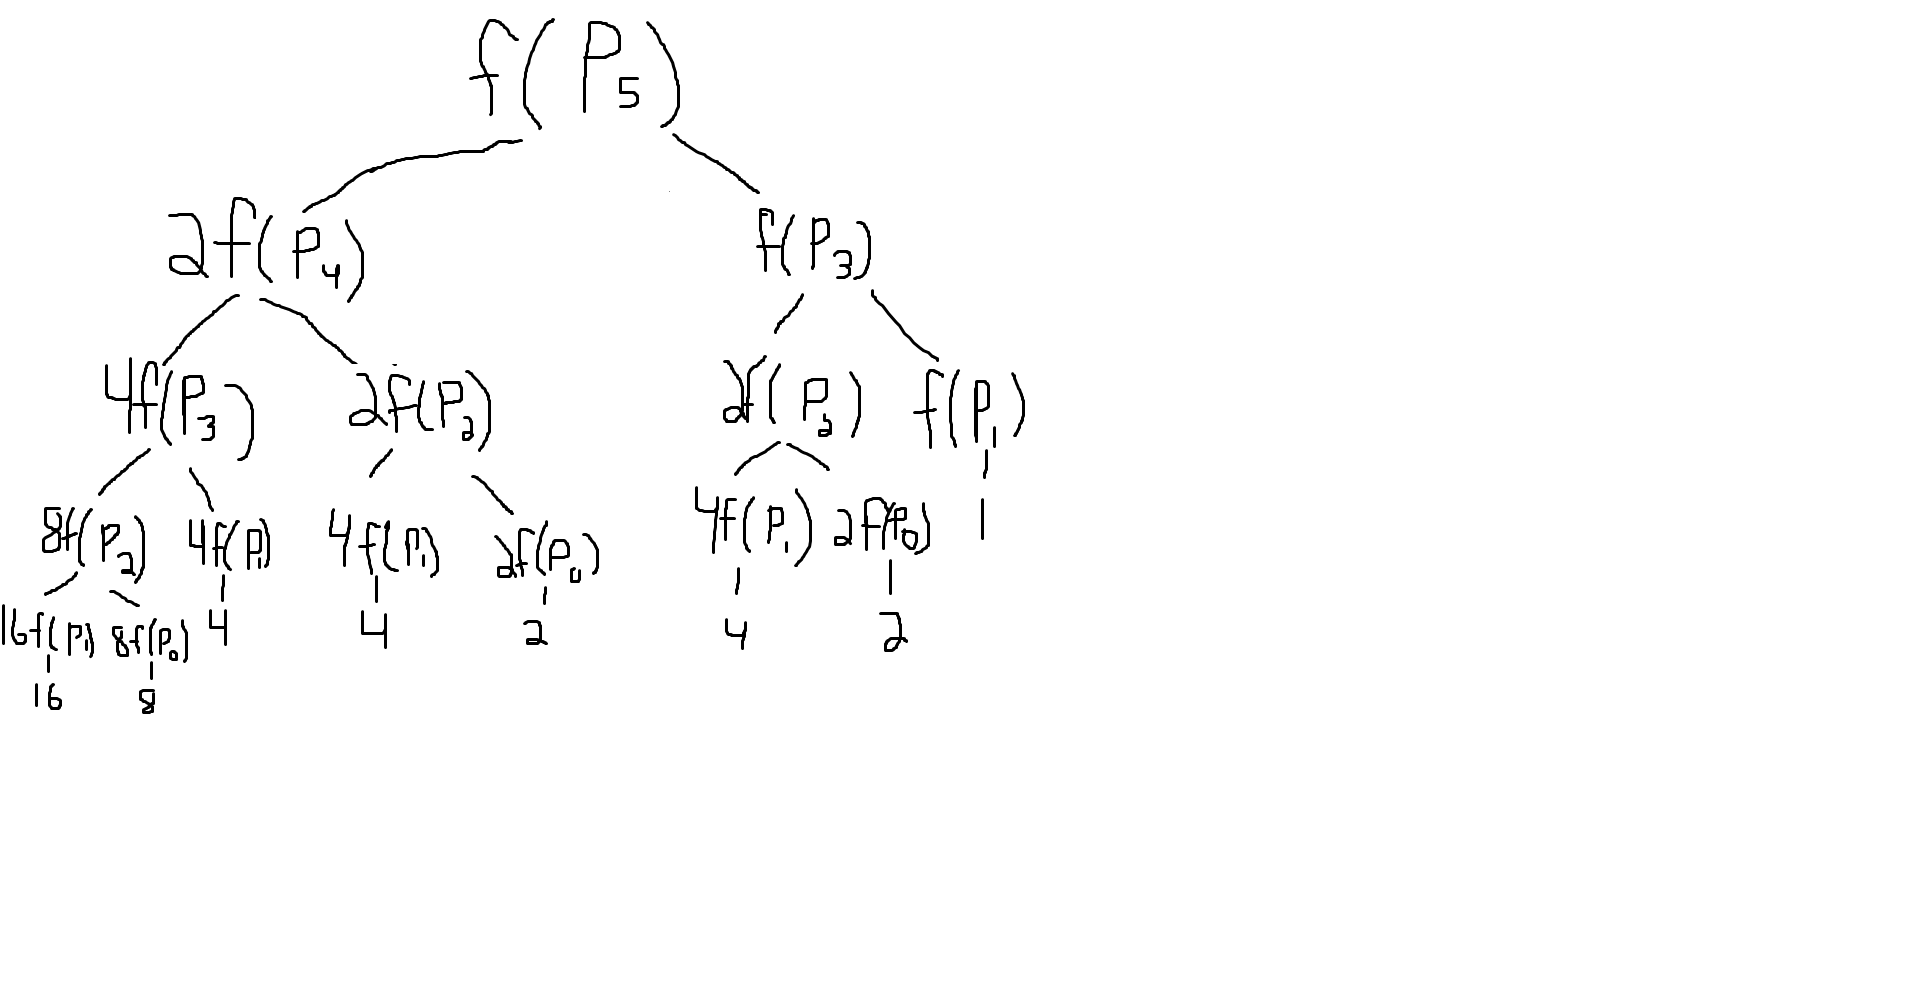
\includegraphics[scale=0.3]{TreeRec}$ 
    \end{solution}
	
	\item Write down the recurrence for the running time $T(n)$ of the algorithm.\\
% 	and solve for it.
	\begin{solution}
$\newline$ T(n)=2T(n-1)+T(n-2)+$O(1)$
    \end{solution}

	\end{enumerate}
		
	\item \label{q:3:memfib} (6 pts) Consider the dynamic programming approach ``top-down implementation with memoization'' that memoizes the intermediate Pell numbers by storing them in an array $P[n]$. 
		
	\begin{enumerate}
	\item Write down an algorithm for the top-down implementation with memoization in pseudocode.  \\
	\begin{solution}
$\newline$ P=[] $\newline$def memo(n): $\newline -->$ if P[n]!=None: $\newline --/-->$ return P[n] $\newline -->$ if n==0 or n==1: $\newline --/-->$ P[n]=1 $\newline -->$ else: $\newline --/-->$ P[n]=2*memo(n-1)+memo(n-2) $\newline -->$ return P[n]
    \end{solution}
	
	\item Draw the tree of function calls to calculate $P_5$. You can call your function $f$ in this diagram.\\
	\begin{solution}
$\newline$ $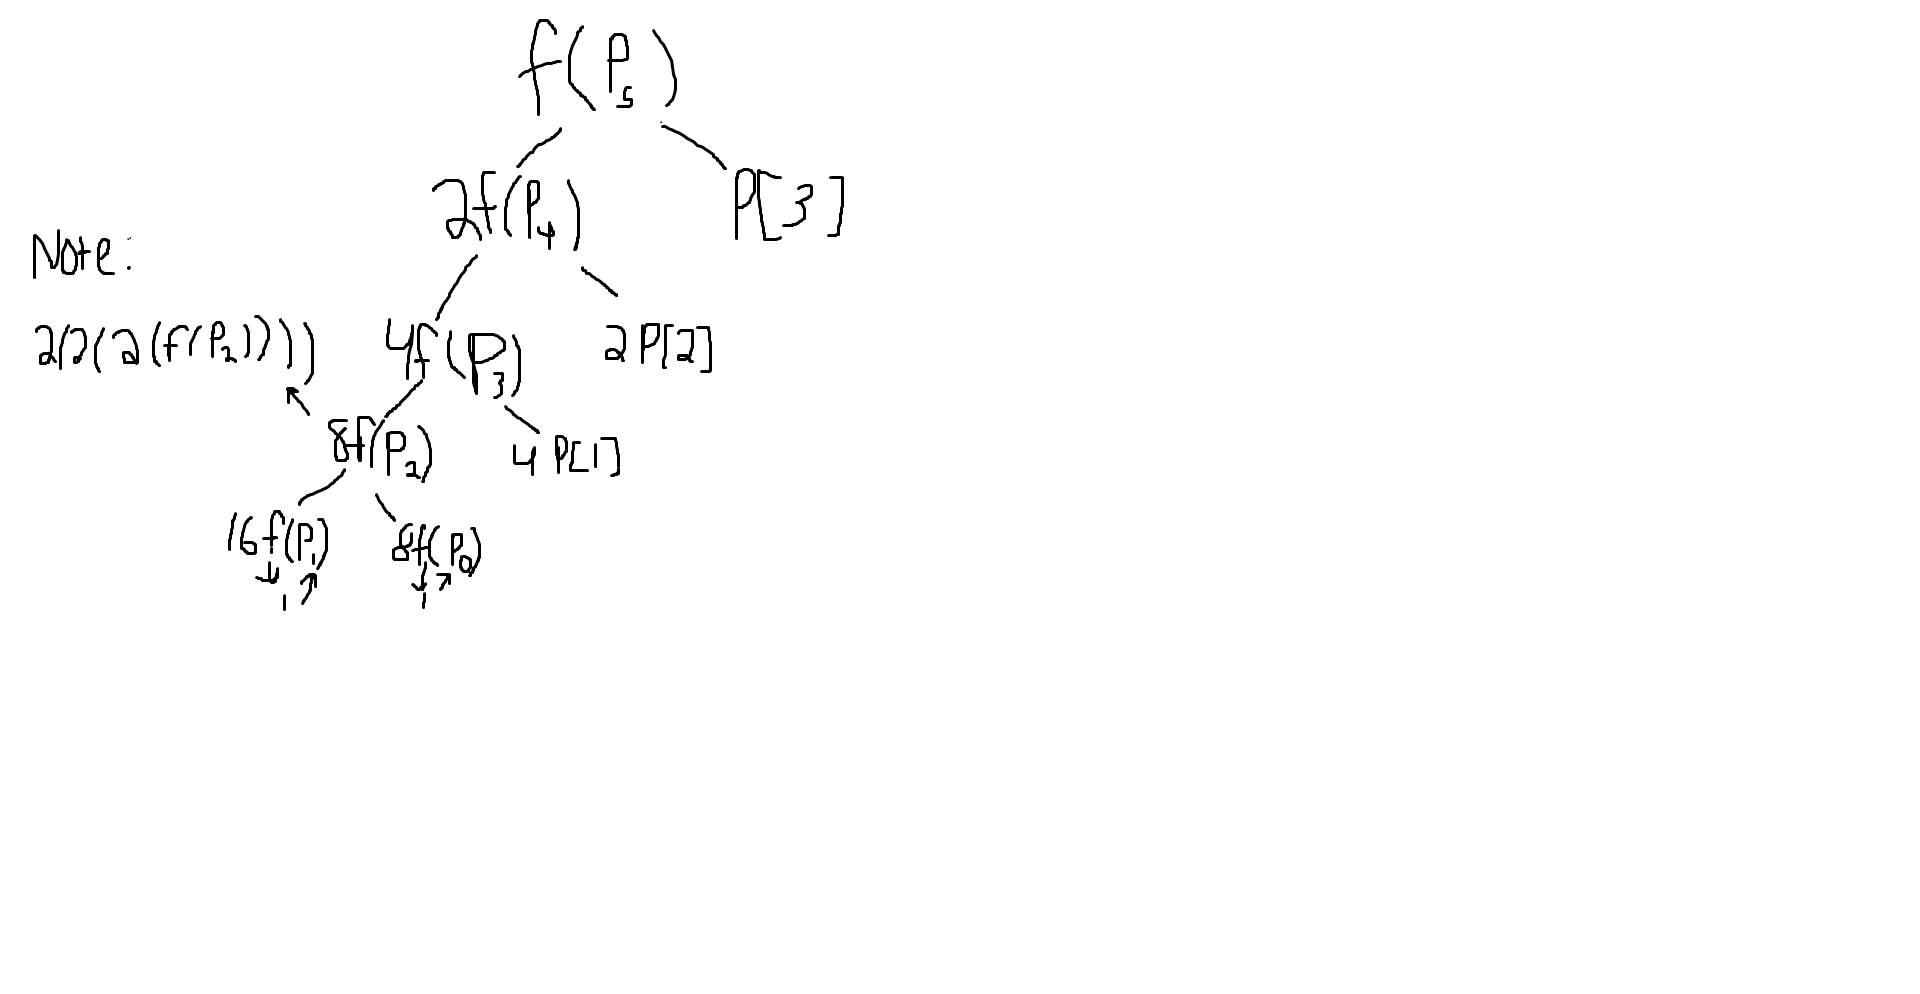
\includegraphics[scale=0.3]{TreeMemo}$
    \end{solution}

	\item In order to find the value of $P_5$, you would fill the array $P$ in a certain order. Provide the order in which you will fill $P$ showing the values. \\
	\begin{solution}
$\newline$ Order: n=1,0,2,3,4,5 (1 and 0 once recursed down, 2 given by 1 and 0, 3 given by 2 and 1, and 4 given by 3 and 2. 4 cannot happen until 3 is done, and so on) for values 1,1,3,7,17,41
    \end{solution}
	

	\item Determine and justify briefly the asymptotic running time $T(n)$ of the algorithm. \\
% 	Prove your claim is correct by induction on the contents of the array.
	\begin{solution}
$\newline$ T(n)=2T(n-1)+$O(1)$ (right side negated by simple call to P) $\newline$ Base Case: $P_0$ and $P_1$ are both 1. No additional calculations needed for them on either side. $\newline$ Inductive Hypothesis: Since the array holds previous answers and the right side is a previous answer to the left, T(k)=2T(k-1)+O(1) $\newline$ Inductive Step: T(k+1)=2T(k)+O(1) $-->$ T(k+1)=4T(k-1)+O(1) $-->$ 2T(k)=4T(k-1)+O(1) $-->$ T(k)=T(k-1)+O(1)  $\newline$ Therefore, the relation holds
    \end{solution}
	
	\end{enumerate}
	
	\item (5 pts) Consider the dynamic programming approach ``iterative bottom-up implementation'' that builds up directly to the final solution by filling the $P$ array in order. 	
	\begin{enumerate}
	\item Write down an algorithm for the iterative bottom-up implementation in pseudocode.  \\
    \begin{solution}
$\newline$ def bottom(n): $\newline -->$ P=[] $\newline -->$ for i in range(0,n): $\newline --/-->$ if i==0 or i==1: $\newline --/--/-->$ P.append(1) $\newline --/-->$ else: $\newline --/--/-->$ P.append(2*P[i-1]+P[i-2]) $\newline -->$ return P[n]
    \end{solution}
    
    \item In order to find the value of $P_5$, you would fill the array $P$ in a certain order using this approach. Provide the order in which you will fill $P$ showing the values. \\
    \begin{solution}
$\newline$ This is iterative, so P fills in the order of the iterator i. It goes 0,1,2 (from 0 and 1),3,4,5, for values 1,1,3,7,17,41.
    \end{solution}
    
	\item Determine and justify briefly the time and space usage of the algorithm. \\
	\begin{solution}
$\newline$ This builds with a single for loop from 0-n, which means it has a time complexity of $\Theta(n)$. The array also is just as long as the for loop, so it must have a space complexity of $\Theta(n)$ as well
    \end{solution}
% 	Justify your answers and compare them to the answers in part~\eqref{q:3:memfib}.\\
	
	

	\end{enumerate}

	
	\item \label{q:3:memfid}  (3 pts) If you only want to calculate $P_n$, you can have an iterative bottom-up implementation with $\Theta(1)$ space usage.  Write down an iterative algorithm with $\Theta(1)$ space usage in pseudocode for calculating $P_n$. There is no requirement for the runtime complexity of your algorithm. Justify your algorithm does have $\Theta(1)$ space usage.
    \begin{solution}
$\newline$ def theta(n): $\newline -->$ P=1 $\newline -->$ c=1 $\newline -->$ d=1 $\newline -->$ for i in range(2,n): $\newline --/-->$ P=2*c+d $\newline --/-->$ d=c $\newline --/-->$ c=P $\newline -->$ return P $\newline \newline$ This is space $\Theta(1)$ because it only temporarily holds previous values in the form of c (our i-1) and d (our i-2), not actually using any more space than a few variables, which is not one, but it is BIG THETA of 1 as it does not change depending on how many n there is.
    \end{solution}
	
	
	\item (2 pts) In a table, list each of the four algorithms as rows and in separate columns, provide each algorithm's asymptotic time and space requirements. Briefly discuss how these different approaches compare, and where the improvements come from.
	\begin{solution}
$\newline$ $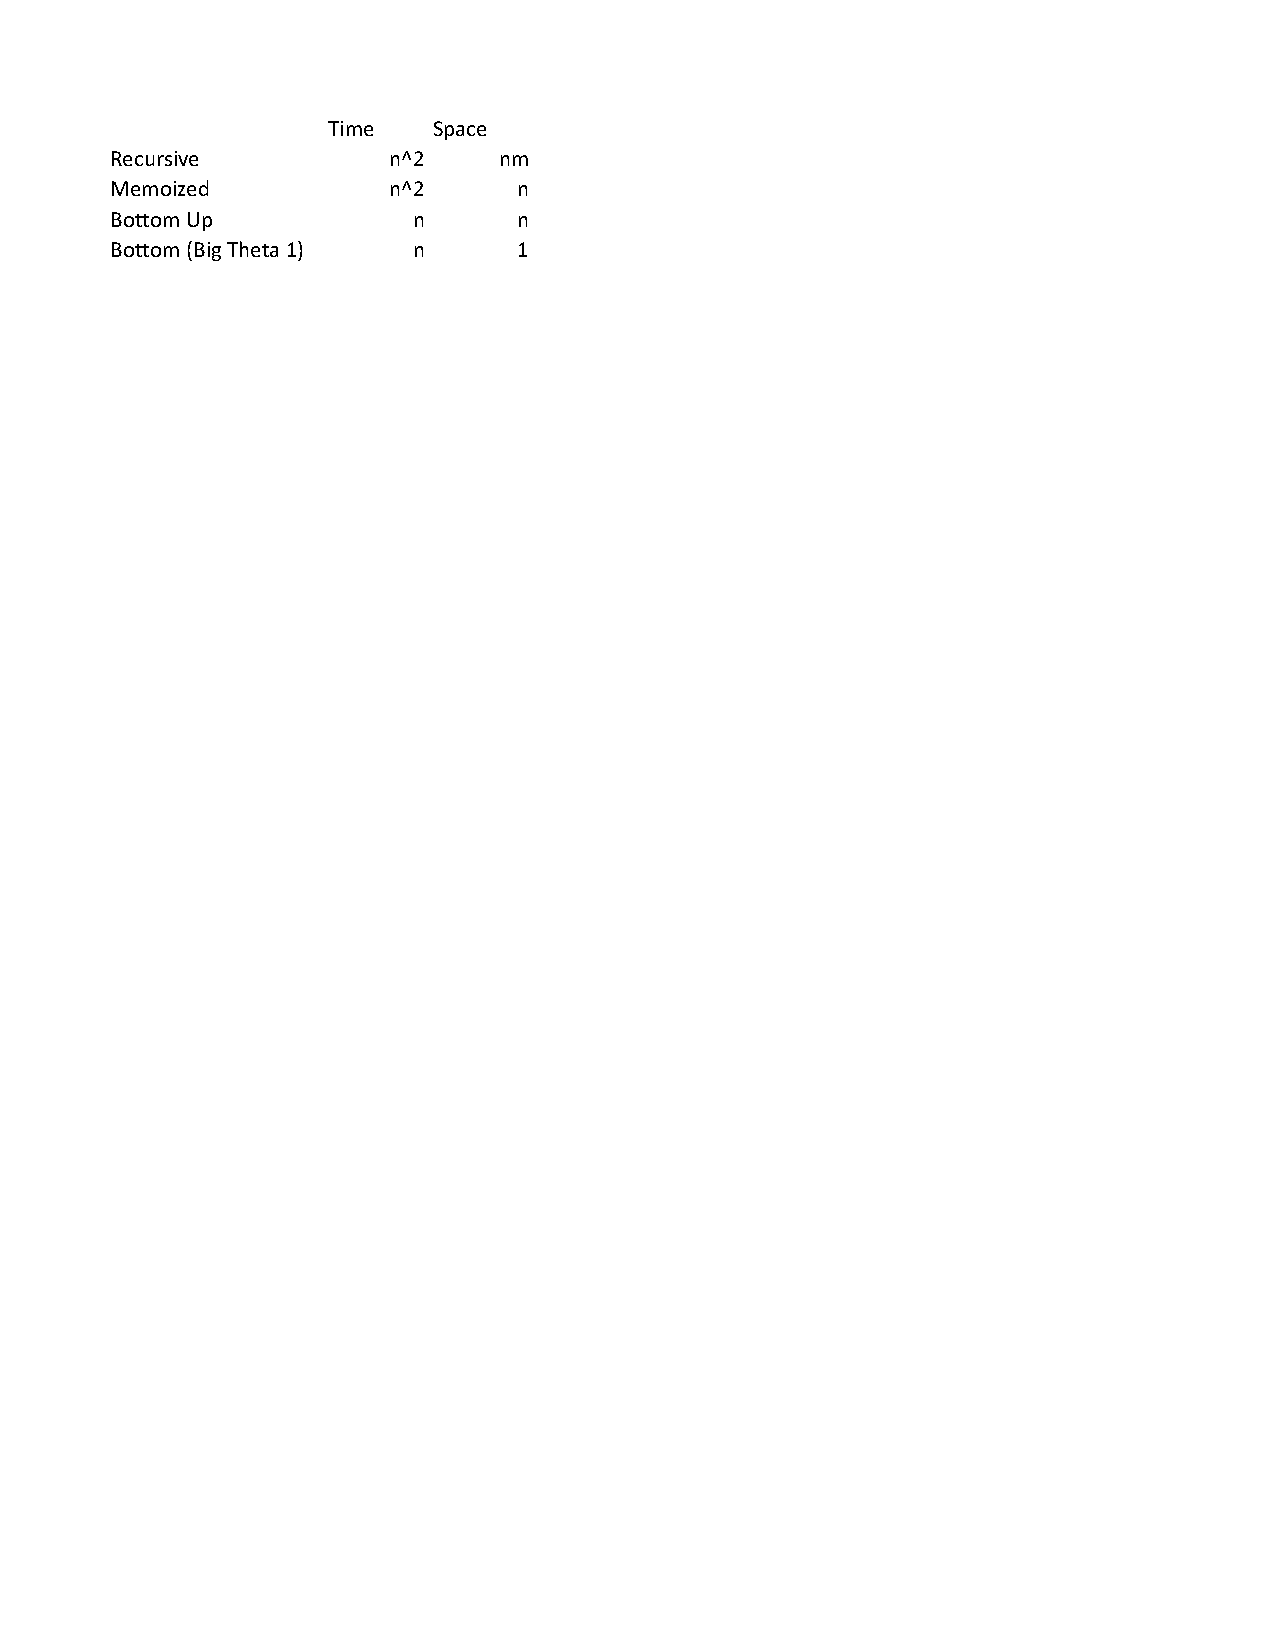
\includegraphics[scale=0.9]{Book22}$ $\newline$ The recursive has cuts on both the left and right at each level, meaning it takes a total space of mn (n depth passed in times m splits per level). Time T(n) has two splits as well, however, due to the similarity of each side, the time merges together to make a wopping $n^2$, which comes from the unrolling of T(n-1) $->$ T(n-k)+n(k-1)+(k-1), k=n. $\newline$ The Memoized version also has a recursive relation, but it goes down only one side. Though it does not need to merge a n-2 term, it still groups to a time complexity of $n^2$. However, the lack of a right side makes it take less space. In this case, it would be $\frac{1}{2}$ mn, and since there are two splits, this becomes just n space. It needs to go through each n to get the overall solution still, but storing values gives it no need to go through right sides. $\newline$ The bottom-up approach does not deal with the weirdness that comes with recursive trees. It uses a loop instead of recursive calls, still making for stored values without the breakoff. This means the time only relies on the loop to fill the array and space relies purely on the array (as previous values are just pulled from the array we already calculated). $\newline$ The bottom-up $\Theta(1)$ version inherits a lot of the benefits of the regular bottom-up, in that it only relies on a loop. This one, however, only stores a little in the form of variables, assuming the loop is sequential. It only uses a few variables to store some of the most recent instead of holding a whole array, which makes its scope pretty small, but makes the space complexity only the variables, and as such, $\Theta(1)$.
    \end{solution}


	\end{enumerate}
    \pagebreak

    \item (10 pts) Write a single python code for the following. There is a very busy student at CU who is taking CSCI 3104. They know that this course has a ton of homework and they don't want to attempt all of the homework. This student cherishes the downtime and has \textbf{decided not to do any two consecutive assignments}.
    \\
    Assume that the student gets a list of assignments with the points associated at the beginning of the semester. Use dynamic programming to pick which assignments to complete to maximize the available points while not solving any two consecutive assignments. 
    
    Input: [2,7,9,3,1]\\
    Output: 12\\
    Explanation: Maximum points available = 2 + 9 + 1 = 12.\\
    
    
    
    \begin{enumerate}
        \item (2 pts) Show an example with at least $4$ assignments to show why the greedy strategy \\ $max( sum( even\_indexed\_terms) , sum ( odd\_indexed\_term))$ does not work.\\
        Example - For the above list, $sum( even\_indexed\_terms) = 2+9+1$ and \\ $sum( even\_indexed\_terms) = 7+3$. But, coincidentally their $max$ gives out the optimal answer. You have to provide an example where this doesn't work.
        \begin{solution}
$\newline$ Array: $\newline$
[ 20   6  13 100  11   2] $\newline$
Optimal: $\newline$
[20, 100, 2] $\newline$
122 $\newline$
Greedy: $\newline$
[6, 100, 2] $\newline$
108 $\newline \newline$ The greedy takes advantage of that 100, but it ignores the 20 to choose the 6, leading to a non-optimal solution
        \end{solution}
        
        % \item (4 pts) Write a recursive function that takes the list of assignments and outputs the maximum points that the student can attempt. 
        % \item (4 pts) Write the top-down memoization based version for part (a).
        \item (4 pts) Write the bottom-up DP table filling version that takes the list of assignments and outputs the maximum points that the student can attempt. (If it helps, you can code the recursive approach for practice but you don't need to submit that)
        
        \item (4 pts) Write the DP version for part (b) which uses $O(1)$ space.
        
        
        \textbf{Note that you don't have to submit anything for part (b) and (c) on the pdf but only the commented code in the python file.}
    \end{enumerate}



    
    


\pagebreak



\item (10 pts) Suppose we are trying to create an optimal health shake from a number of ingredients, which we label $\mathcal{I} = \{1, \ldots, n\}$. Each cup of an ingredient contributes $p_{i}$ units of protein, as well as $c_{i}$ calories. Our goal is to maximize the amount of protein, such that the shake uses no more than $C$ calories. \textbf{Note that you can use more than one cup of each ingredient.} 
\begin{itemize}
    \item Design an DP based algorithm which takes the arrays $p$ and $c$ and calories $C$ as input and outputs the maximum protein you can put using no more than $C$ calories.
    \item In order to fill a particular table entry, you would need to access some sub-problems. Explain briefly which decisions each of those sub-problems represent.
    \item Also, provide the runtime and space requirement of your algorithm.
\end{itemize}
 
\begin{solution}
$\newline$ def calories(p,c,C): $\newline -->$ arr=[][] (Assume this is initialized 2D list)  $\newline -->$ if len(c)==0 or C==0:  $\newline --/-->$ return 0  $\newline -->$ for i in range(0,C):  $\newline --/-->$ for j in range(0,len(c)):  $\newline --/--/-->$ if j==0 or i==0:  $\newline --/--/--/-->$ arr[i][j]=0  $\newline --/--/-->$ elif c[j]$>$i:  $\newline --/--/--/-->$ arr[i][j]=arr[i][j-1] $\newline --/--/-->$ else: $\newline --/--/--/-->$ m=max(arr[i][j-1], p[j]+arr[i-c[j]][j-1]) $\newline --/--/--/-->$ arr[i][j]=m $\newline --/--/--/-->$ if m!=arr[i][j-1]: $\newline --/--/--/--/-->$ j-=1 $\newline -->$ return arr[C][len(c)] $\newline$ Subproblems represent the maximum protein amount for previous calorie counts. These subproblems are used to build on the previous protein amounts, as adding some to a previous best case now that we are allowing more calories helps us by not having to figure it all out again just with less restriction. $\newline$ The runtime is C*len(c), which is basically $n^2$ by concept because of the two loops, but the two do not use the same n, and thus must reflect that in the notation. Space is the exact same, as it fills the whole array to the sizes given by the loops (as the highest protein is the point at [C][len(c)], or [Calorie count][num items]).
\end{solution}

\pagebreak
\item (10 pts) In recitation you learnt the longest common sub-sequence (LCS) problem, where you used a DP table to find the length of the LCS and to recover the LCS (there might be more than one LCS of equal length).
For example - For two sequences $X = \{A, B, C, B, D, A, B\}$ and $Y = \{B, D, C, A, B, A\}$. Here's a complete solution. Grey cells represent one of the LCS (BCBA) and the red-bordered cells represent another (BCAB). Note that you have to provide only one optimal solution.

% ----- FIGURE -----
\begin{figure}[h!]
\begin{center}
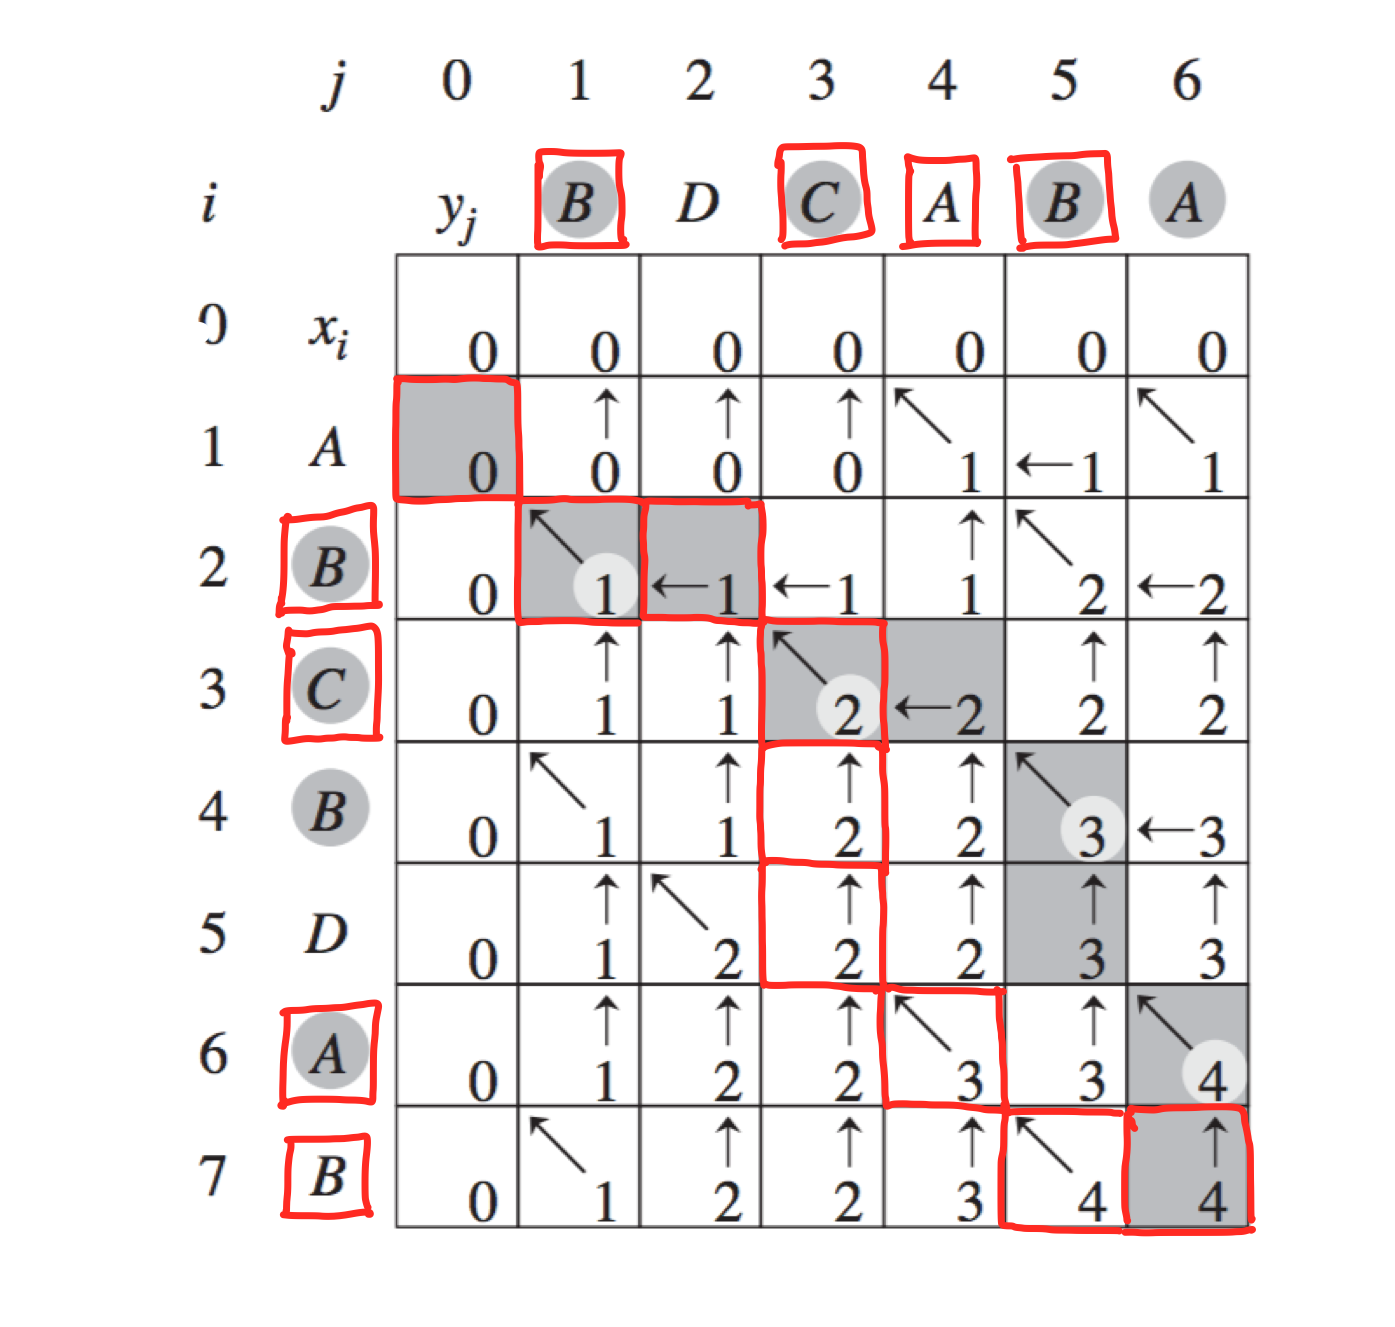
\includegraphics[scale=0.3]{LCS.jpeg} 
\end{center}
\end{figure}
% ----------

\begin{enumerate}
    \item (6 pts) Draw the complete table for $X = \{A,B,A,C,D\}$ and $Y = \{B,A,D,B,C,A\}$.
    \begin{itemize}
        \item Fill in all the values and parent arrows.
        \item Backtrack and circle all the relevant cells to recover the actual LCS and not only the length. Do not forget to circle the appropriate characters too.
        \item Report the length of the LCS and the actual LCS.
    \end{itemize}
    
    \begin{solution}
$\newline$ $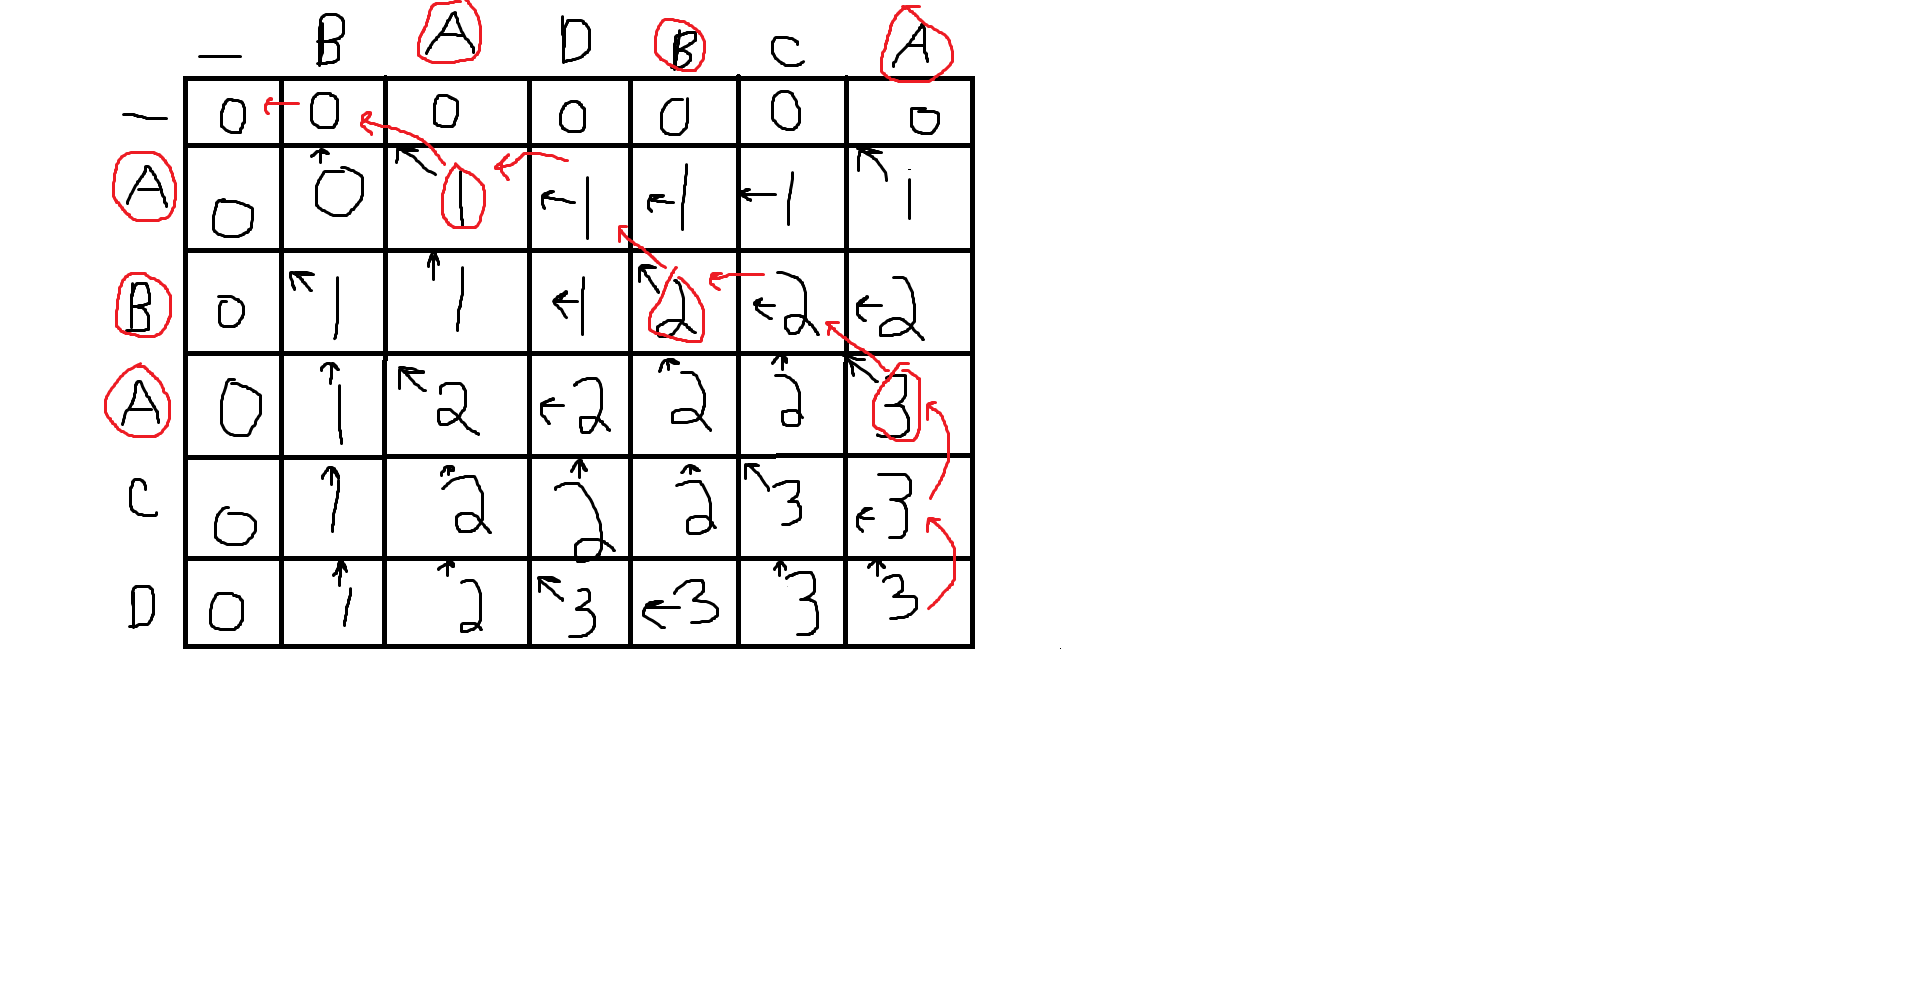
\includegraphics[scale=0.7]{DPTab} $ $\newline$ Length: 3, LCS: ABA
    \end{solution}
    
    
    \pagebreak
    \item (4 pts) If you draw the recursive tree for the recursive version of LCS, you will get something like this.
    % ----- FIGURE -----
\begin{figure}[h!]
\begin{center}
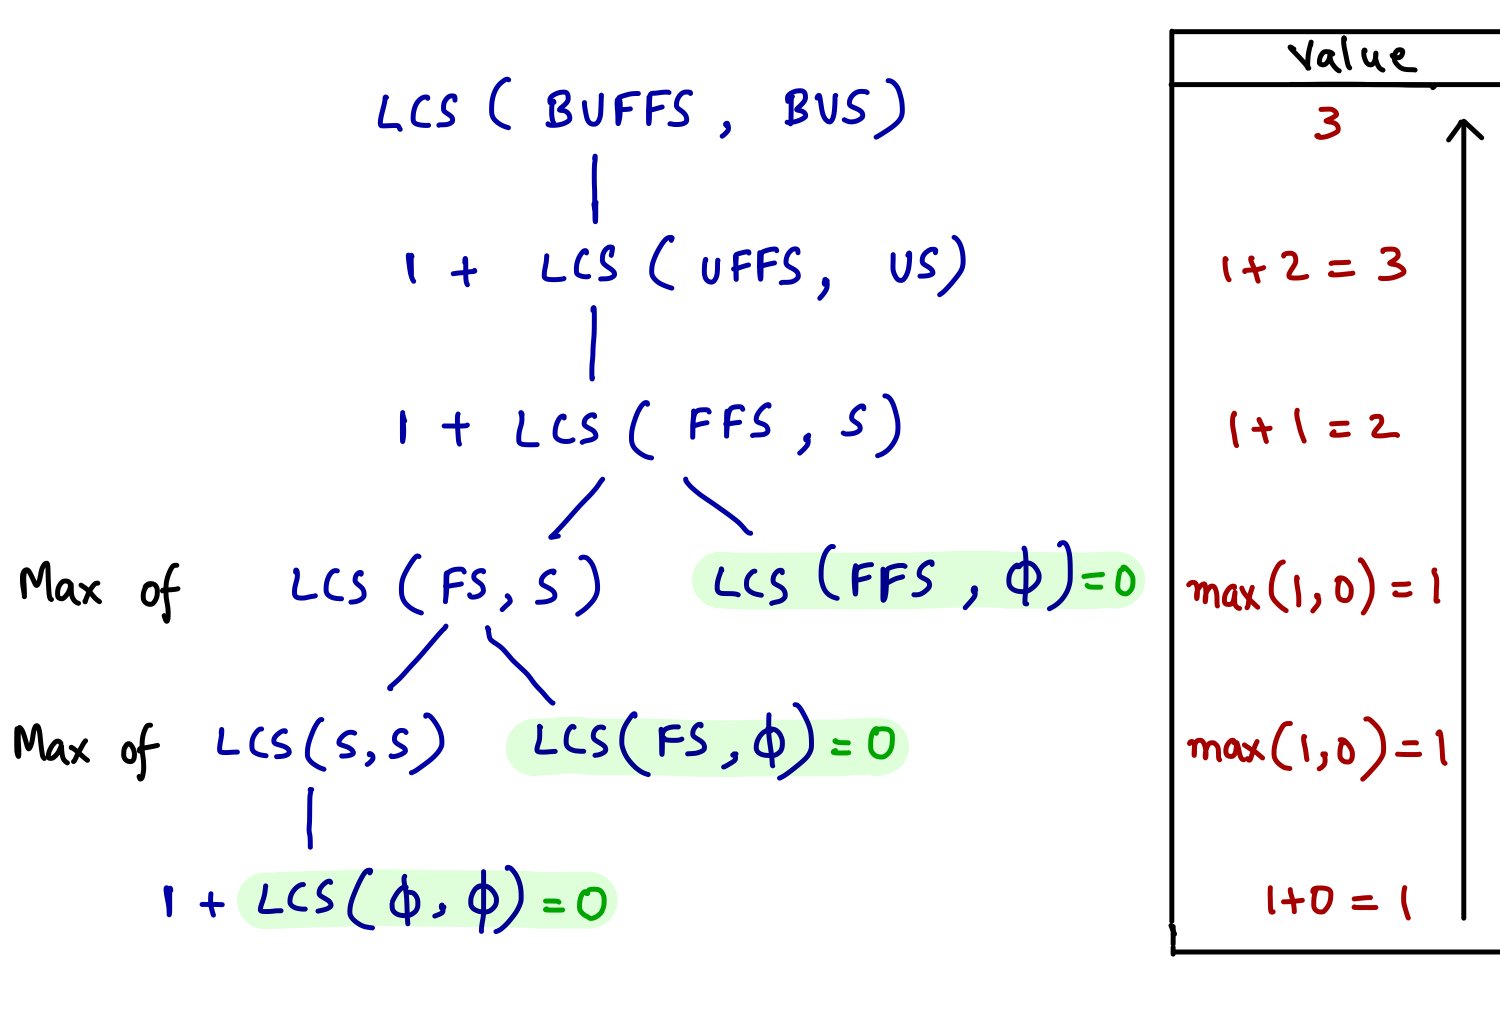
\includegraphics[scale=0.3]{LCS_recursive.jpeg} 
\end{center}
\end{figure}
% --
Here we show all the recursive calls till the base case and annotate the children calls with a $'Max'$ or a $'+1'$ while indicating the base case calls. 
We also compute the values from bottom to top as we get them. 
Draw a tree like above for the LCS calls for string $'SFUB'$ and $'SUB'$ i.e. $LCS( SFUB, SUB ) $.

\begin{solution}
$\newline$$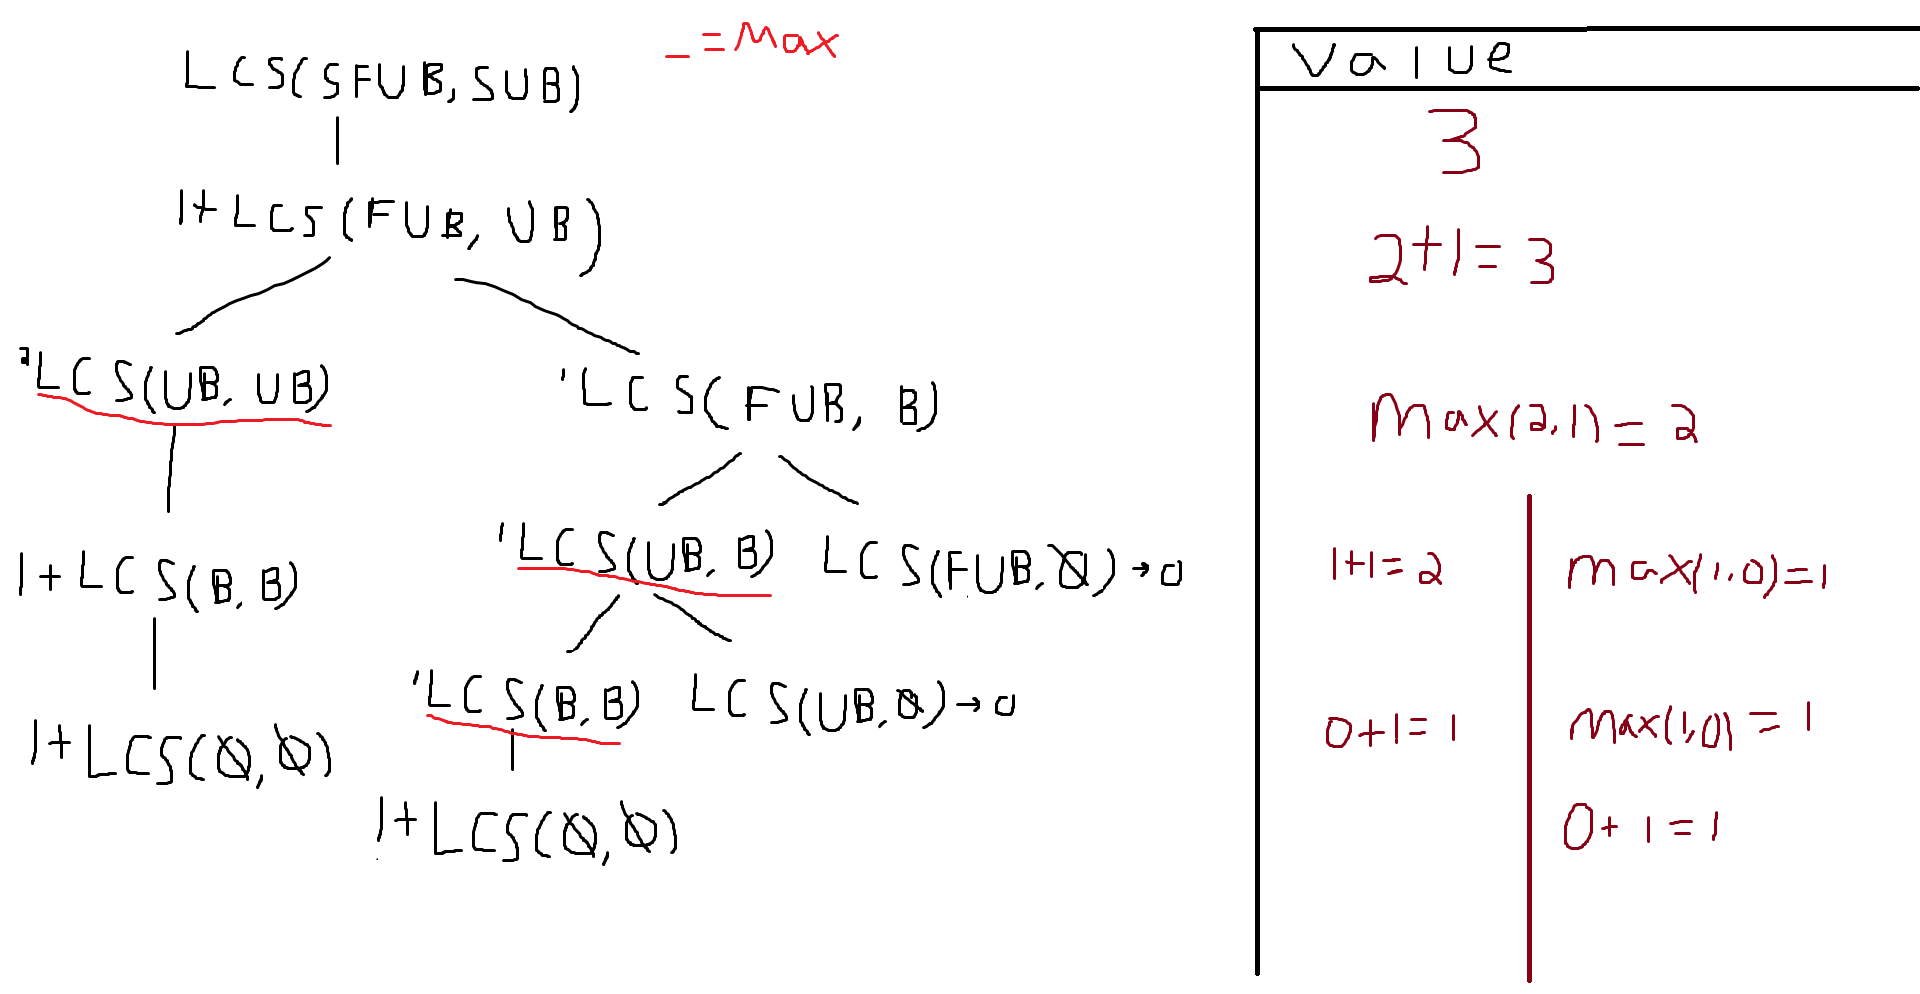
\includegraphics[scale=0.3]{RecTree} $
\end{solution}

\end{enumerate}
    
    
\end{enumerate}


\end{document}


